\chapter{Results}\label{ch:Results}
This chapter presents the simulation results and a comparison between all proposed methods in different scenarios variating from low to high weed density infestation. The goal of this chapter is to come up with the best solution for the task allocation problem and measure the performance improvement over the baseline method.

Paltech currently offers its weeding solutions in fields ranging from $0.5$ to $20$ hectares, with an average weed density of $0.4$ to $1.0$ weeds/m$^2$. \autoref{fig:field-weed-density} shows an example of usual weed density in a 1-hectare field, while \autoref{fig:field-path-planning} illustrates the coverage path planning pattern that the robot follows in the same field. The simulations in this thesis are limited to the linear movements shown in \ref{fig:field-path-planning}, due to the motion constraints described at the beginning of chapter \ref{ch:TA}. As a result, the simulation environments were designed accordingly.

\begin{figure}[htb]
    \myfloatalign
    \subfloat[Weed density]
    {\label{fig:field-weed-density}
        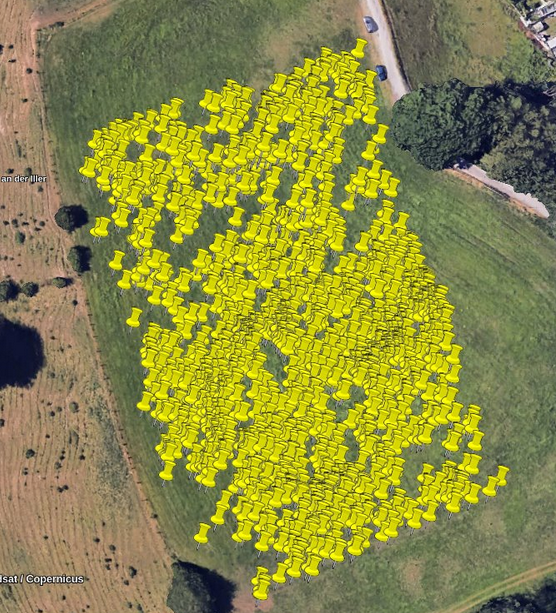
\includegraphics[width=.41\linewidth]{gfx/ch04/field_weed_density.png}} \quad
    \subfloat[Coverage path planning pattern]
    {\label{fig:field-path-planning}%
        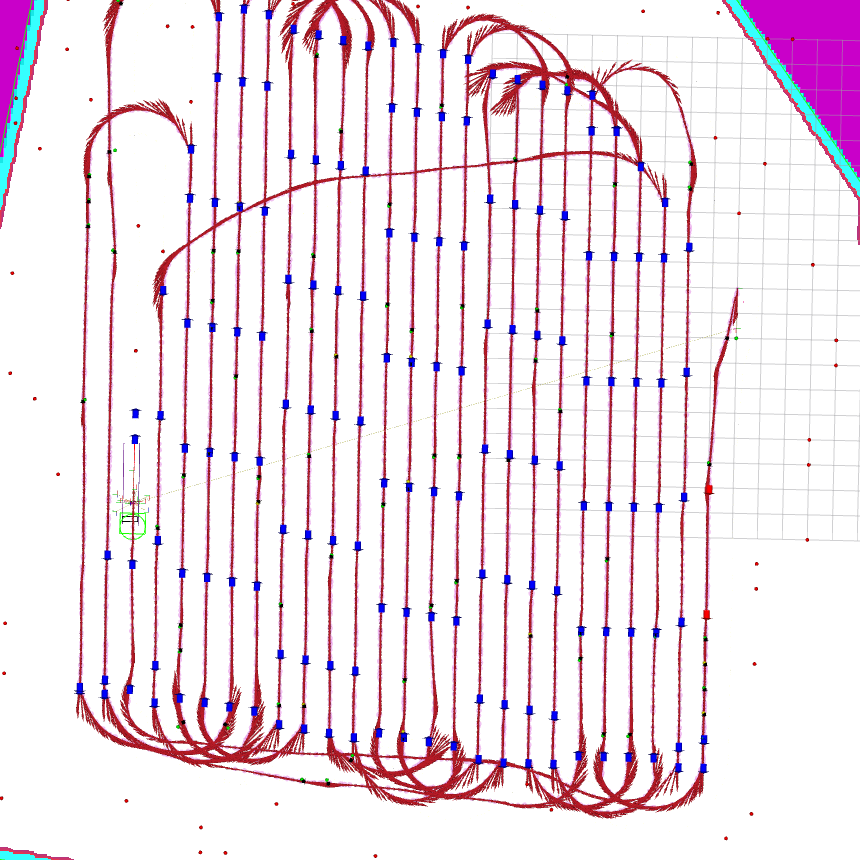
\includegraphics[width=.45\linewidth]{gfx/ch04/field_path_planning.png}} \\
    \caption{Weed distribution and coverage path in an agricultural field}\label{fig:usual-field-example}
\end{figure}

\section{Simulation Setup}
Simulations were customized using YAML files, as mentioned in \autoref{sec:simulation}, allowing for ease of configuration and logging convenience. All tests took place in a rectangular grass field of $10\text{m} \times 50\text{m}$, with different weed densities along a straight strip of $2\text{m} \times 50\text{m}$, simulating one line of the coverage path planning (observe an example in \autoref{fig:sim-example}). The local weed distribution within each quadrant ($2\text{m} \times 2\text{m}$) varied in both type (\textit{uniform} or \textit{clustered}) and density, replicating irregular Rumex growth. 

\begin{figure}[hbt]
    \centering
    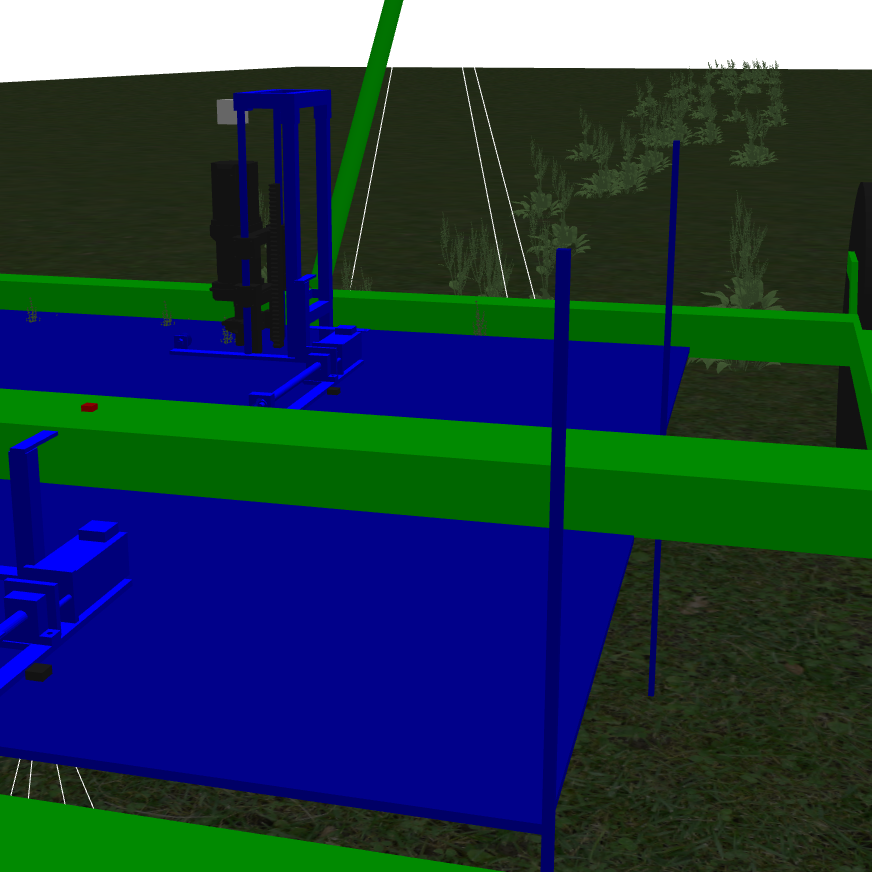
\includegraphics[width=0.5\linewidth]{gfx/ch04/field_strip_path_2.png}
    \caption{Simulation Example}
    \label{fig:sim-example}
\end{figure}

\section{Algorithm Comparison}
The first simulation corresponds to an infestation area of $100\text{m}^2$, with a weed density of $0.28$ weeds/m$^2$. This simulates a low weed density scenario, as shown in \autoref{fig:task-visualization-low-density}. \autoref{fig:results-low-density} presents both the task visualization and the mission metrics comparison across algorithms. 

The first two missions in \autoref{fig:mission-metrics-low-density} represent the baseline method using one and two tools, respectively. This comparison was made only to determine the natural improvement in mission time when adding an additional tool, even with a non-optimized algorithm. Missions three, four, and five correspond to the graph search, optimization, and market-based approaches, respectively. We observe similar mission times and no significant improvement over the baseline method, which is expected since the weed density is low and, most of the time, the separation between weeds prevents the robot from reaching them with both tools simultaneously. Nevertheless, we observe a reduction in tool idle time with algorithms three, four, and five. The heuristic algorithm results in an idle time of $12.8$ min. for the front tool, whereas the others remain within the range of $8$ min. to $9.8$ min.

\begin{figure}[htb]
    \myfloatalign
    \subfloat[Task Visualization]
    {\label{fig:task-visualization-low-density}
        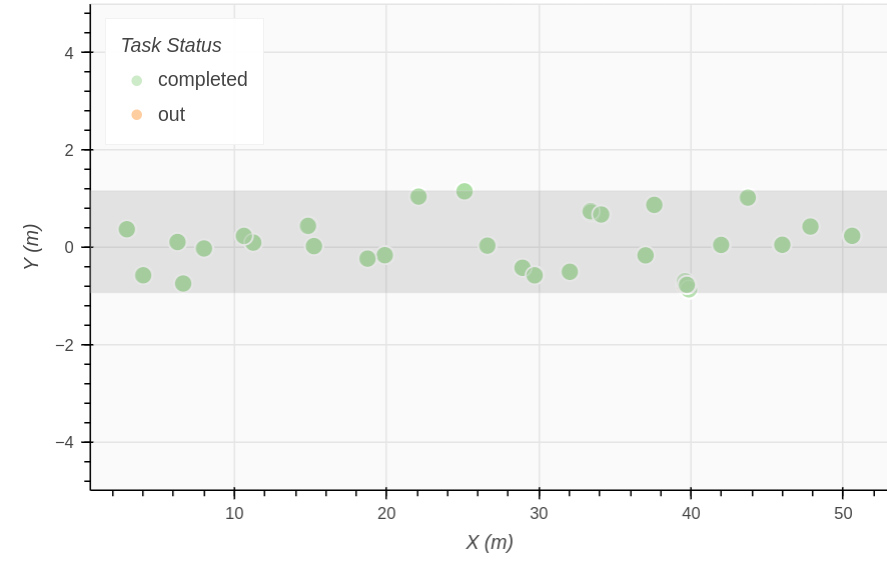
\includegraphics[width=.45\linewidth]{gfx/ch04/50m_low_density_tasks.png}} \quad
    \subfloat[Mission Metrics]
    {\label{fig:mission-metrics-low-density}
        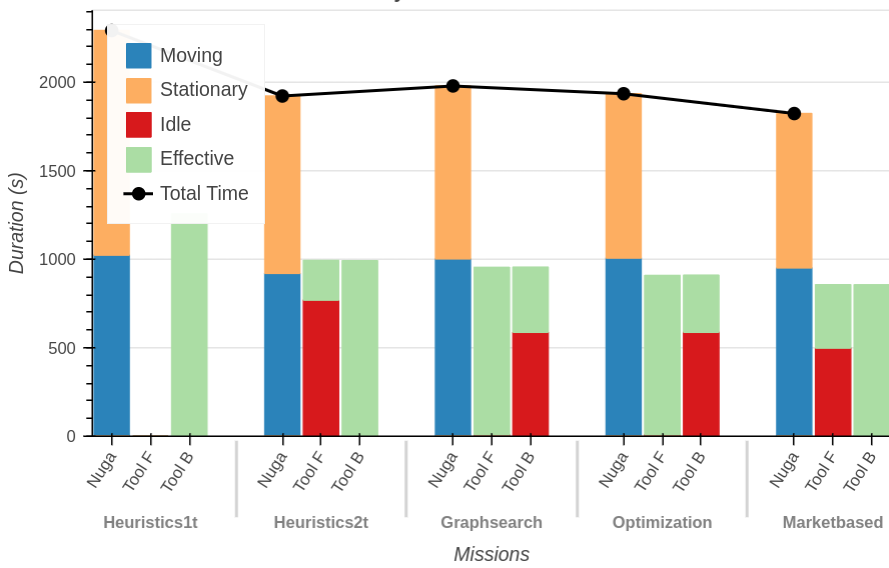
\includegraphics[width=.45\linewidth]{gfx/ch04/50m_low_density_missions.png}} \\
    \caption{Low density algorithms comparison}\label{fig:results-low-density}
\end{figure}

For the second simulation, we increased the average weed density to $0.55$ weeds/m$^2$, simulating a medium-density scenario, as shown in \autoref{fig:task-visualization-medium-density}. In \autoref{fig:mission-metrics-medium-density}, we observe improvements in both mission time and tool productivity. Both the graph search and optimization-based algorithms show improvements compared to the heuristic approach. Specifically, while the baseline method overuses the back tool, resulting in high idle time for the front tool, graph search and optimization achieve more balanced tool usage. The market-based algorithm also reduces idle time, although not as significantly as the other two methods.

\begin{figure}[htb]
    \myfloatalign
    \subfloat[Task Visualization]
    {\label{fig:task-visualization-medium-density}
        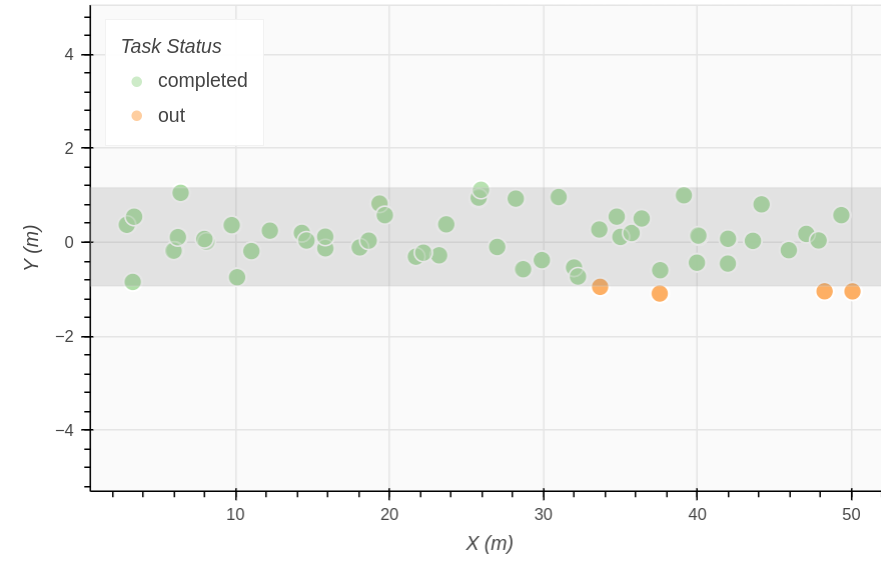
\includegraphics[width=.45\linewidth]{gfx/ch04/50m_medium_density_tasks.png}} \quad
    \subfloat[Mission Metrics]
    {\label{fig:mission-metrics-medium-density}
        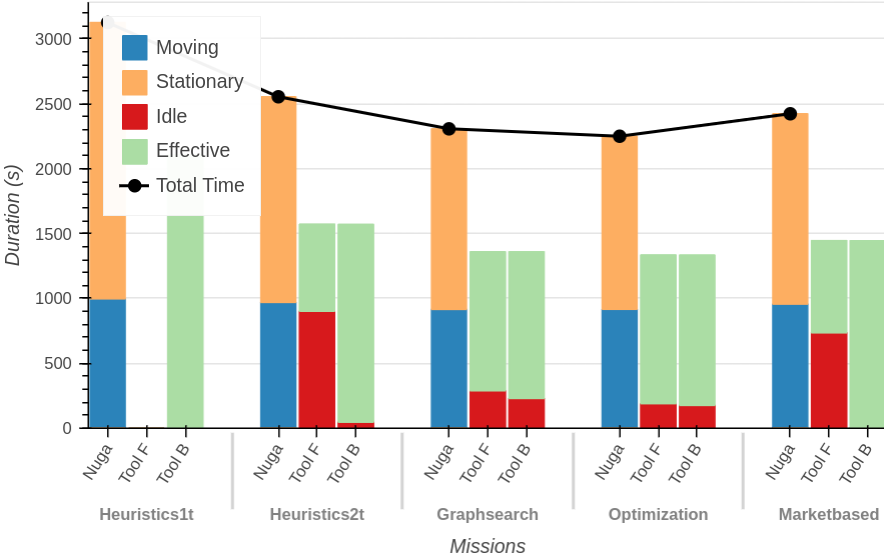
\includegraphics[width=.45\linewidth]{gfx/ch04/50m_medium_density_missions.png}} \\
    \caption{Medium density algorithms comparison}\label{fig:results-medium-density}
\end{figure}

The third simulation corresponds to a weed density of $1.55$ weeds/m$^2$, simulating a high-density scenario, as shown in \autoref{fig:task-visualization-high-density}. Similar to the medium-density scenario (but more pronounced) the graph search and optimization-based approaches show better performance by reducing both mission time and idle time for both tools, achieving balanced tool usage. The market-based algorithm also shows noticeable improvements, achieving better tool productivity and mission time reduction than the baseline, although it still lags behind the other two methods.

\begin{figure}[htb]
    \myfloatalign
    \subfloat[Task Visualization]
    {\label{fig:task-visualization-high-density}
        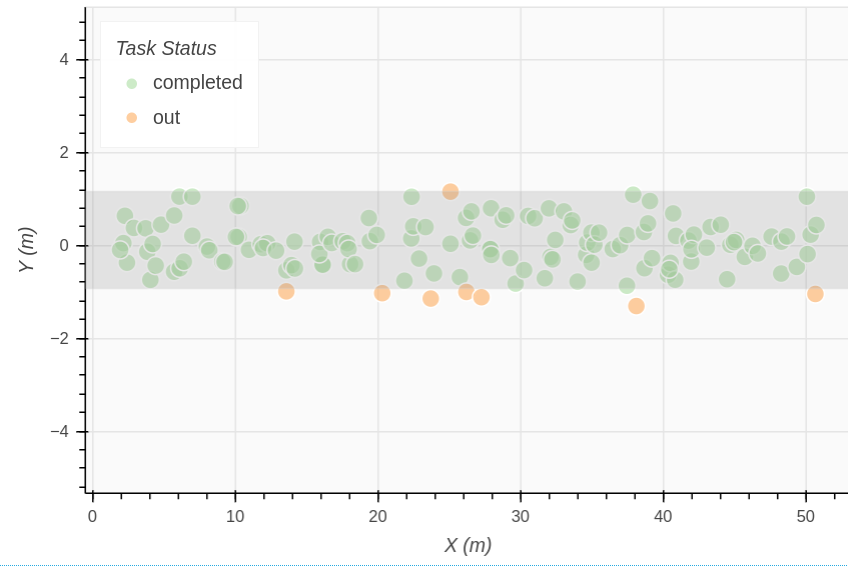
\includegraphics[width=.45\linewidth]{gfx/ch04/50m_high_density_tasks.png}} \quad
    \subfloat[Mission Metrics]
    {\label{fig:mission-metrics-high-density}
        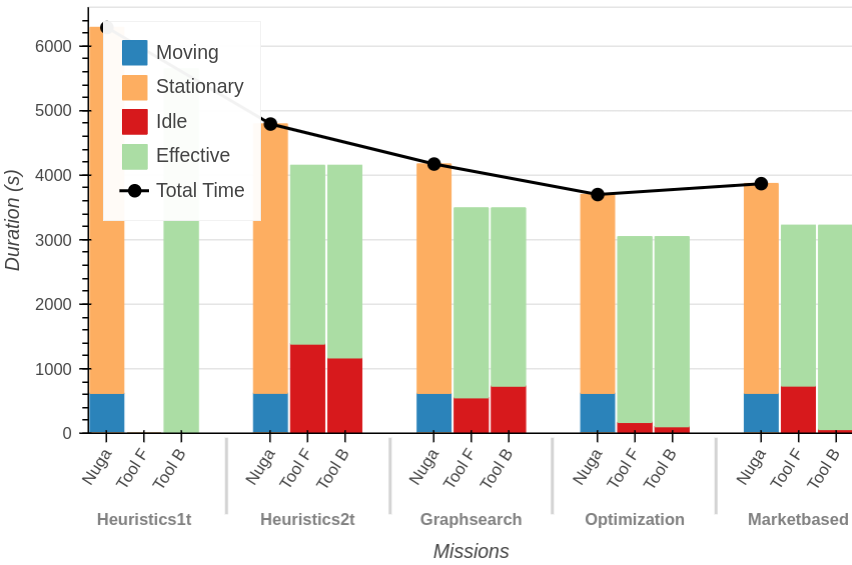
\includegraphics[width=.45\linewidth]{gfx/ch04/50m_high_density_missions.png}} \\
    \caption{High density algorithms comparison}\label{fig:results-high-density}
\end{figure}

The simulation results are summarized in \autoref{tab:low-results}, \autoref{tab:medium-results}, \autoref{tab:high-results} for the low, medium, and high-density simulations, respectively. Each table presents the same information as the previous bar graphs under the '\textit{Raw}' column. Additionally, the '\textit{Improvement}' column shows the relative percentage difference of each algorithm compared to the baseline method for each category. This allows to determine the best algorithm for each weed density scenario.

\begin{table}[H]
    \centering
    \begin{tblr}{
      row{5} = {Silver},
      row{7} = {Silver},
      row{11} = {Silver},
      row{13} = {Silver},
      cell{1}{3} = {c=5}{c},
      cell{1}{8} = {c=5}{c},
      cell{3}{1} = {r=3}{},
      cell{3}{2} = {Silver},
      cell{3}{3} = {Silver},
      cell{3}{4} = {Silver},
      cell{3}{5} = {Silver},
      cell{3}{6} = {Silver},
      cell{3}{7} = {Silver},
      cell{3}{8} = {Silver},
      cell{3}{9} = {Silver},
      cell{3}{10} = {Silver},
      cell{3}{11} = {Silver},
      cell{3}{12} = {Silver},
      cell{6}{1} = {r=3}{},
      cell{6}{8} = {fg=red},
      cell{6}{9} = {fg=JapaneseLaurel},
      cell{6}{10} = {fg=red},
      cell{7}{11} = {fg=JapaneseLaurel},
      cell{7}{12} = {fg=JapaneseLaurel},
      cell{8}{11} = {fg=red},
      cell{8}{12} = {fg=red},
      cell{9}{1} = {r=3}{},
      cell{9}{2} = {Silver},
      cell{9}{3} = {Silver},
      cell{9}{4} = {Silver},
      cell{9}{5} = {Silver},
      cell{9}{6} = {Silver},
      cell{9}{7} = {Silver},
      cell{9}{8} = {Silver,fg=red},
      cell{9}{9} = {Silver,fg=JapaneseLaurel},
      cell{9}{10} = {Silver,fg=red},
      cell{9}{11} = {Silver},
      cell{9}{12} = {Silver},
      cell{10}{11} = {fg=JapaneseLaurel},
      cell{10}{12} = {fg=JapaneseLaurel},
      cell{11}{11} = {fg=red},
      cell{11}{12} = {fg=red},
      cell{12}{1} = {r=3}{},
      cell{12}{8} = {fg=red},
      cell{12}{9} = {fg=JapaneseLaurel},
      cell{12}{10} = {fg=JapaneseLaurel},
      cell{13}{11} = {fg=JapaneseLaurel},
      cell{13}{12} = {fg=JapaneseLaurel},
      cell{14}{12} = {fg=red},
    }
                                               &    & Raw (min) &       &       &      &      & Improvement (\%) &       &       &        &       \\
                                               &    & Mov.      & Stat. & Total & Idle & Eff. & Mov.             & Stat. & Total & Idle   & Eff.  \\
    \begin{sideways}Heuristics\end{sideways}   & N  & 15.3      & 16.7  & 32    & -    & -    & -                & -     & -     & -      & -     \\
                                               & FT & -         & -     & -     & 12.8 & 3.7  & -                & -     & -     & -      & -     \\
                                               & BT & -         & -     & -     & 0.1  & 16.4 & -                & -     & -     & -      & -     \\
    \begin{sideways}Graph Search\end{sideways} & N  & 16.7      & 16.2  & 32.9  & -    & -    & 9.2              & -3.0  & 2.8   & -      & -     \\
                                               & FT & -         & -     & -     & 0.1  & 15.7 & -                & -     & -     & -99.2  & 324.3 \\
                                               & BT & -         & -     & -     & 9.8  & 6.1  & -                & -     & -     & 9700.0 & -62.8 \\
    \begin{sideways}Optimization\end{sideways} & N  & 16.7      & 15.4  & 32.2  & -    & -    & 9.2              & -7.8  & 0.6   & -      & -     \\
                                               & FT & -         & -     & -     & 0.1  & 14.9 & -                & -     & -     & -99.2  & 302.7 \\
                                               & BT & -         & -     & -     & 9.8  & 5.3  & -                & -     & -     & 9700.0 & -67.7 \\
    \begin{sideways}Market\end{sideways}       & N  & 15.8      & 14.5  & 30.3  & -    & -    & 3.3              & -13.2 & -5.3  & -      & -     \\
                                               & FT & -         & -     & -     & 8.3  & 5.9  & -                & -     & -     & -35.2  & 59.5  \\
                                               & BT & -         & -     & -     & 0.1  & 14.2 & -                & -     & -     & 0.0    & -13.4 
    \end{tblr}
    \caption{Low-density Simulation Results}
    \label{tab:low-results}
\end{table}

\paragraph{\autoref{tab:low-results}} Illustrates the convention used to represent the graph. 

\begin{table}[H]
    \centering
    \begin{tblr}{
      row{5} = {Silver},
      row{7} = {Silver},
      row{11} = {Silver},
      row{13} = {Silver},
      cell{1}{3} = {c=5}{c},
      cell{1}{8} = {c=5}{c},
      cell{3}{1} = {r=3}{},
      cell{3}{2} = {Silver},
      cell{3}{3} = {Silver},
      cell{3}{4} = {Silver},
      cell{3}{5} = {Silver},
      cell{3}{6} = {Silver},
      cell{3}{7} = {Silver},
      cell{3}{8} = {Silver},
      cell{3}{9} = {Silver},
      cell{3}{10} = {Silver},
      cell{3}{11} = {Silver},
      cell{3}{12} = {Silver},
      cell{6}{1} = {r=3}{},
      cell{6}{8} = {fg=JapaneseLaurel},
      cell{6}{9} = {fg=JapaneseLaurel},
      cell{6}{10} = {fg=JapaneseLaurel},
      cell{7}{11} = {fg=JapaneseLaurel},
      cell{7}{12} = {fg=JapaneseLaurel},
      cell{8}{11} = {fg=red},
      cell{8}{12} = {fg=red},
      cell{9}{1} = {r=3}{},
      cell{9}{2} = {Silver},
      cell{9}{3} = {Silver},
      cell{9}{4} = {Silver},
      cell{9}{5} = {Silver},
      cell{9}{6} = {Silver},
      cell{9}{7} = {Silver},
      cell{9}{8} = {Silver,fg=JapaneseLaurel},
      cell{9}{9} = {Silver,fg=JapaneseLaurel},
      cell{9}{10} = {Silver,fg=JapaneseLaurel},
      cell{9}{11} = {Silver},
      cell{9}{12} = {Silver},
      cell{10}{11} = {fg=JapaneseLaurel},
      cell{10}{12} = {fg=JapaneseLaurel},
      cell{11}{11} = {fg=red},
      cell{11}{12} = {fg=red},
      cell{12}{1} = {r=3}{},
      cell{12}{8} = {fg=JapaneseLaurel},
      cell{12}{9} = {fg=JapaneseLaurel},
      cell{12}{10} = {fg=JapaneseLaurel},
      cell{13}{11} = {fg=JapaneseLaurel},
      cell{13}{12} = {fg=JapaneseLaurel},
      cell{14}{11} = {fg=JapaneseLaurel},
      cell{14}{12} = {fg=red},
    }
                                               &    & Raw (min) &       &       &      &      & Improvement (\%) &       &       &        &       \\
                                               &    & Mov.      & Stat. & Total & Idle & Eff. & Mov.             & Stat. & Total & Idle   & Eff.  \\
    \begin{sideways}Heuristics\end{sideways}   & N  & 16.1      & 26.4  & 42.5  & -    & -    & -                & -     & -     & -      & -     \\
                                               & FT & -         & -     & -     & 15   & 11.1 & -                & -     & -     & -      & -     \\
                                               & BT & -         & -     & -     & 0.7  & 25.3 & -                & -     & -     & -      & -     \\
    \begin{sideways}Graph Search\end{sideways} & N  & 15.2      & 23.1  & 38.4  & -    & -    & -5.6             & -12.5 & -9.6  & -      & -     \\
                                               & FT & -         & -     & -     & 4.8  & 17.8 & -                & -     & -     & -68.0  & 60.4  \\
                                               & BT & -         & -     & -     & 3.8  & 18.8 & -                & -     & -     & 442.9  & -25.7 \\
    \begin{sideways}Optimization\end{sideways} & N  & 16        & 24.5  & 40.6  & -    & -    & -0.6             & -7.2  & -4.5  & -      & -     \\
                                               & FT & -         & -     & -     & 1.7  & 22.4 & -                & -     & -     & -88.7  & 101.8 \\
                                               & BT & -         & -     & -     & 9.8  & 14.2 & -                & -     & -     & 1300.0 & -43.9 \\
    \begin{sideways}Market\end{sideways}       & N  & 15.9      & 24.4  & 40.3  & -    & -    & -1.2             & -7.6  & -5.2  & -      & -     \\
                                               & FT & -         & -     & -     & 12.2 & 11.8 & -                & -     & -     & -18.7  & 6.3   \\
                                               & BT & -         & -     & -     & 0    & 24   & -                & -     & -     & -100.0 & -5.1  
    \end{tblr}
    \caption{Medium-density Simulation Results}
    \label{tab:medium-results}
\end{table}

\begin{table}[H]
    \centering
    \begin{tblr}{
      row{4} = {c},
      row{5} = {Silver,c},
      row{7} = {Silver,c},
      row{8} = {c},
      row{10} = {c},
      row{11} = {Silver,c},
      row{13} = {Silver,c},
      row{14} = {c},
      cell{1}{3} = {c=5}{c},
      cell{1}{8} = {c=5}{c},
      cell{3}{1} = {r=3}{},
      cell{3}{2} = {Silver,c},
      cell{3}{3} = {Silver,c},
      cell{3}{4} = {Silver,c},
      cell{3}{5} = {Silver,c},
      cell{3}{6} = {Silver,c},
      cell{3}{7} = {Silver,c},
      cell{3}{8} = {Silver,c},
      cell{3}{9} = {Silver,c},
      cell{3}{10} = {Silver,c},
      cell{3}{11} = {Silver,c},
      cell{3}{12} = {Silver,c},
      cell{6}{1} = {r=3}{},
      cell{6}{2} = {c},
      cell{6}{3} = {c},
      cell{6}{4} = {c},
      cell{6}{5} = {c},
      cell{6}{6} = {c},
      cell{6}{7} = {c},
      cell{6}{8} = {c},
      cell{6}{9} = {c,fg=JapaneseLaurel},
      cell{6}{10} = {c,fg=JapaneseLaurel},
      cell{6}{11} = {c},
      cell{6}{12} = {c},
      cell{7}{11} = {fg=JapaneseLaurel},
      cell{7}{12} = {fg=JapaneseLaurel},
      cell{8}{11} = {fg=JapaneseLaurel},
      cell{8}{12} = {fg=red},
      cell{9}{1} = {r=3}{},
      cell{9}{2} = {Silver,c},
      cell{9}{3} = {Silver,c},
      cell{9}{4} = {Silver,c},
      cell{9}{5} = {Silver,c},
      cell{9}{6} = {Silver,c},
      cell{9}{7} = {Silver,c},
      cell{9}{8} = {Silver,c},
      cell{9}{9} = {Silver,c,fg=JapaneseLaurel},
      cell{9}{10} = {Silver,c,fg=JapaneseLaurel},
      cell{9}{11} = {Silver,c},
      cell{9}{12} = {Silver,c},
      cell{10}{11} = {fg=JapaneseLaurel},
      cell{10}{12} = {fg=JapaneseLaurel},
      cell{11}{11} = {fg=JapaneseLaurel},
      cell{11}{12} = {fg=red},
      cell{12}{1} = {r=3}{},
      cell{12}{2} = {c},
      cell{12}{3} = {c},
      cell{12}{4} = {c},
      cell{12}{5} = {c},
      cell{12}{6} = {c},
      cell{12}{7} = {c},
      cell{12}{8} = {c},
      cell{12}{9} = {c,fg=JapaneseLaurel},
      cell{12}{10} = {c,fg=JapaneseLaurel},
      cell{12}{11} = {c},
      cell{12}{12} = {c},
      cell{13}{11} = {fg=JapaneseLaurel},
      cell{13}{12} = {fg=red},
      cell{14}{11} = {fg=JapaneseLaurel},
      cell{14}{12} = {fg=JapaneseLaurel},
    }
                                               &    & Raw (min) &       &       &      &      & Improvement (\%) &       &       &       &       \\
                                               &    & Mov.      & Stat. & Total & Idle & Eff. & Mov.             & Stat. & Total & Idle  & Eff.  \\
    \begin{sideways}Heuristics\end{sideways}   & N  & 10.3      & 69.4  & 79.8  & -    & -    & -                & -     & -     & -     & -     \\
                                               & FT & -         & -     & -     & 23   & 46   & -                & -     & -     & -     & -     \\
                                               & BT & -         & -     & -     & 19.5 & 49.6 & -                & -     & -     & -     & -     \\
    \begin{sideways}Graph Search\end{sideways} & N  & 10.3      & 59.1  & 69.4  & -    & -    & 0.0              & -14.8 & -13.0 & -     & -     \\
                                               & FT & -         & -     & -     & 9.1  & 48.9 & -                & -     & -     & -60.4 & 6.3   \\
                                               & BT & -         & -     & -     & 12.1 & 45.9 & -                & -     & -     & -37.9 & -7.5  \\
    \begin{sideways}Optimization\end{sideways} & N  & 10.3      & 51.2  & 61.6  & -    & -    & 0.0              & -26.2 & -22.8 & -     & -     \\
                                               & FT & -         & -     & -     & 2.8  & 47.8 & -                & -     & -     & -87.8 & 3.9   \\
                                               & BT & -         & -     & -     & 1.7  & 48.9 & -                & -     & -     & -91.3 & -1.4  \\
    \begin{sideways}Market\end{sideways}       & N  & 10.3      & 54    & 64.4  & -    & -    & 0.0              & -22.2 & -19.3 & -     & -     \\
                                               & FT & -         & -     & -     & 12.2 & 41.4 & -                & -     & -     & -47.0 & -10.0 \\
                                               & BT & -         & -     & -     & 1    & 52.6 & -                & -     & -     & -94.9 & 6.0   
    \end{tblr}
    \caption{High-density Simulation Results}
    \label{tab:high-results}
\end{table}